\section{Security of GNSS}

\paragraph{Global Positioning System (GPS):}
\begin{itemize}
    \item 24 satellites at about 20'200 km above earth. Each satellite transmits navigation messages containing its location and precise time of transmission.
    \item Unique pseudorandom codes are used
    \item GPS receiver measures each navigation message's arrival time and estimates its distance to the satellite.
    \item Receivers position and time is calculated using trilateration.
    \item \textbf{C/A (Coarse Acquisition) codes:} (Coarse Acquisition) codes: Gold Codes, 1023 chips, transmitted at 1.023 Mbits (i.e., repeats every 1ms), uses L1 only
    \item \textbf{P (precision) codes:} 6.1871 × $10^{12}$ chips long, transmitted at 10.23 Mbit/s, (i.e. repeats once a week), uses L1 and L2 only
    \item \textbf{Y (P(Y)) code:} encrypted P code (modulated with secret W)
    \item \textcolor{blue}{L1 = 1575.42 MHz, L2 = 1227.60 MHz}
    \item DSSS is used to make the signal more robust (b.c. of distance we end up below noice level at receiver)
\end{itemize}

\begin{minipage}{\linewidth}
    \centering      
    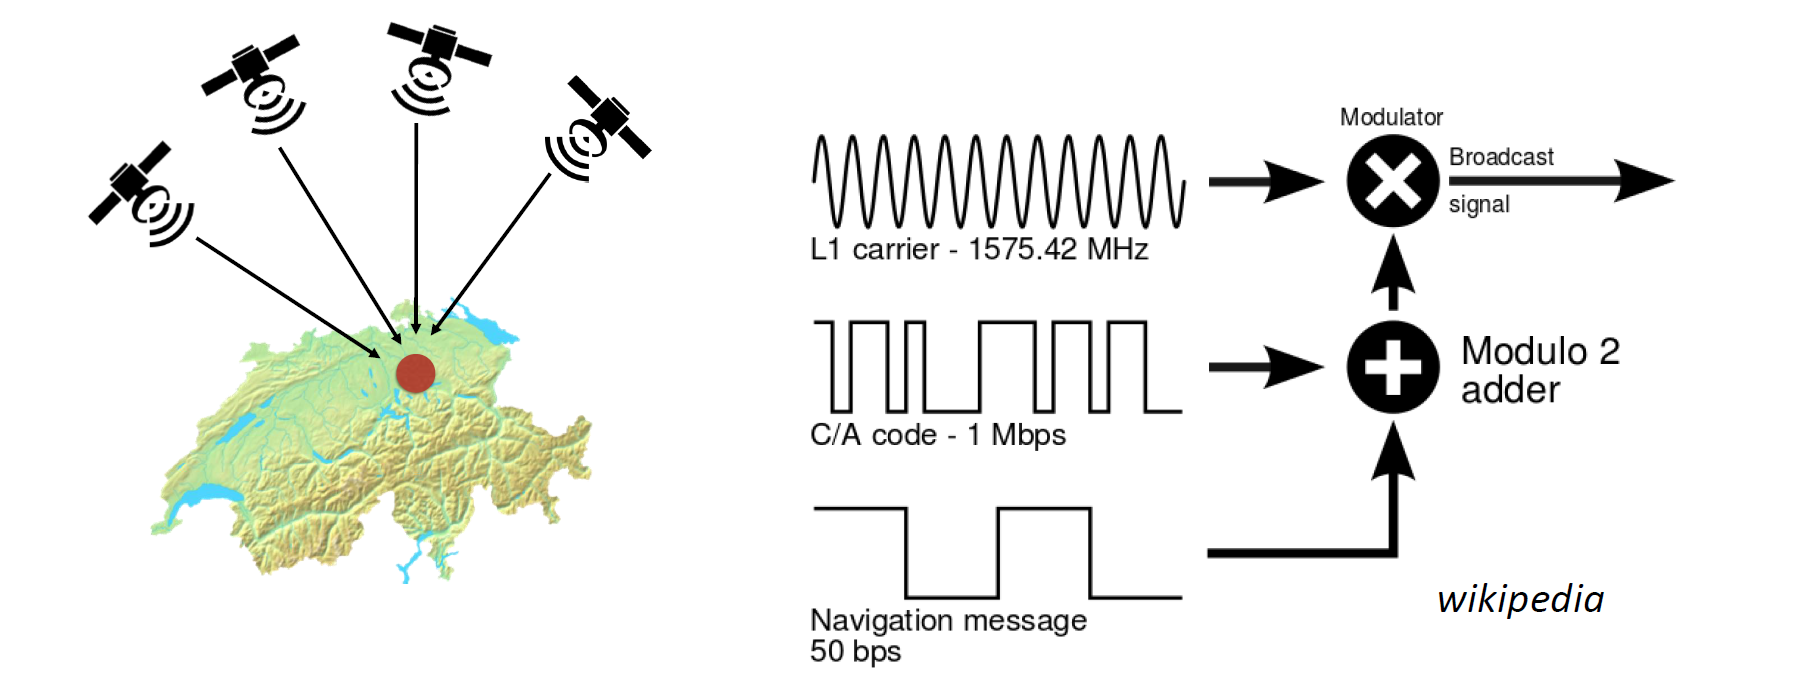
\includegraphics[width=\linewidth]{Figures/L4_gps.PNG} 
\end{minipage}
\begin{minipage}{\linewidth}
    \centering      
    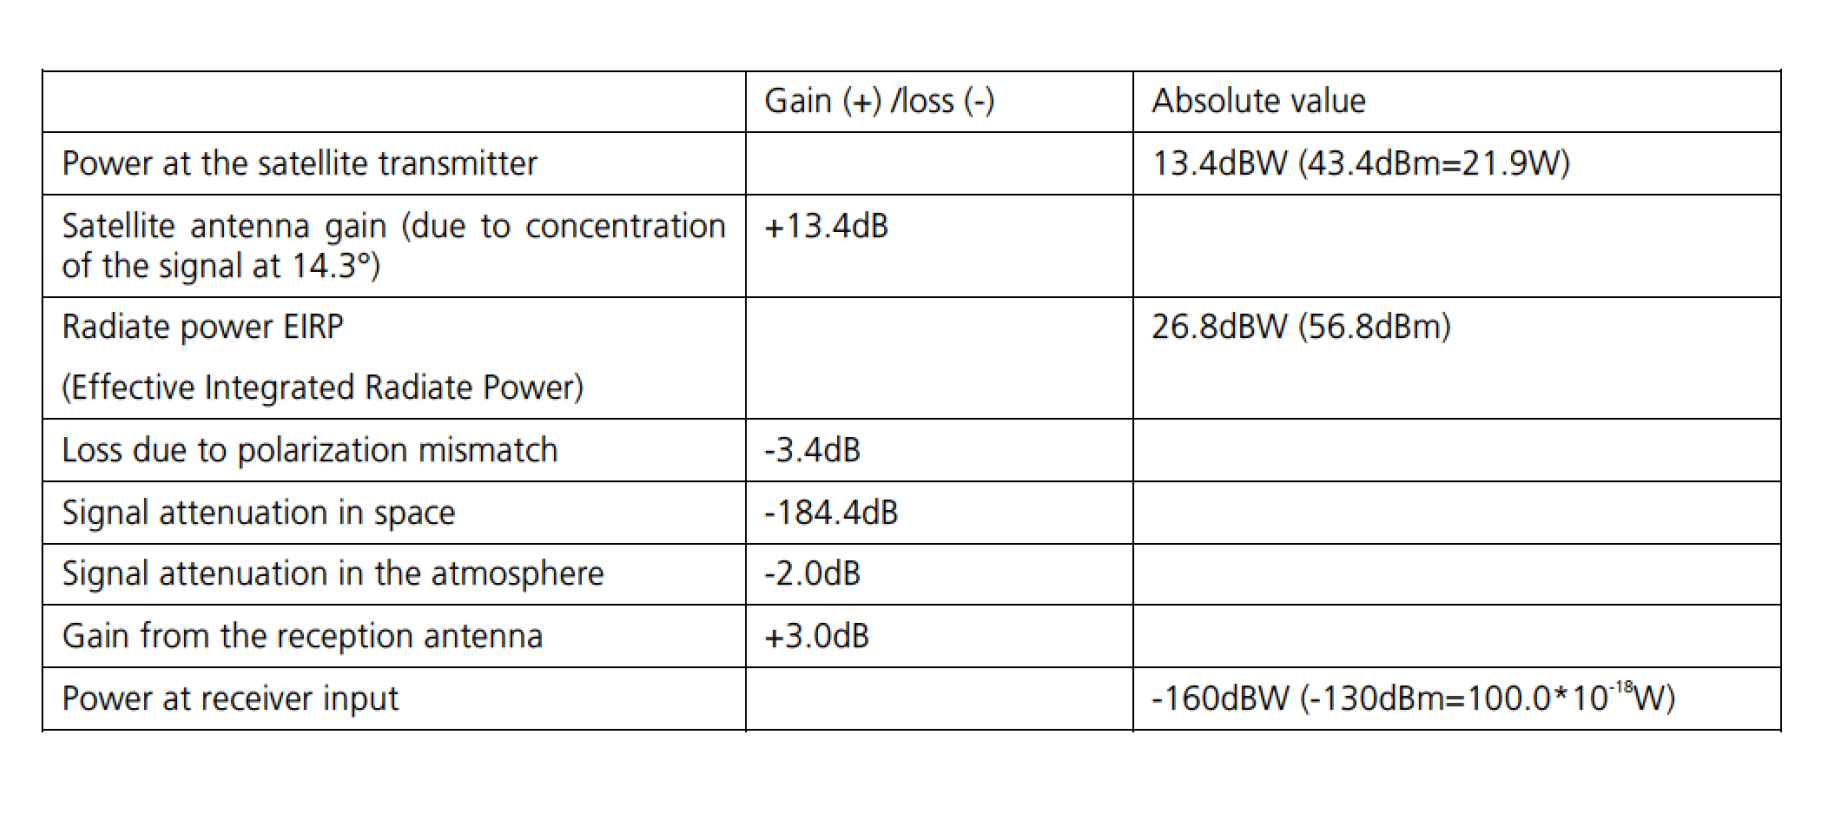
\includegraphics[width=\linewidth]{Figures/L4_power.PNG} 
\end{minipage}

\paragraph{Satellite signal:} The time to transmit all this information is \textbf{12.5 minutes}. By using the navigation message, the receiver is able to determine the transmission time of each satellite signal and the exact position of the satellite at the time of transmission.
\begin{itemize}
    \item Satellite time and synchronization signals
    \item Precise satellite orbital data (ephemeris)
    \item Time correction information to determine the exact satellite time
    \item Approximate orbital data for all satellites (almanac)
    \item Correction signals to calculate signal transit time
    \item Data on the ionosphere
    \item Information on the operating status (health) of the satellite
\end{itemize}

\paragraph{Time of Arrival:} Measuring signal travel times in GPS 
\begin{minipage}{\linewidth}
    \centering      
    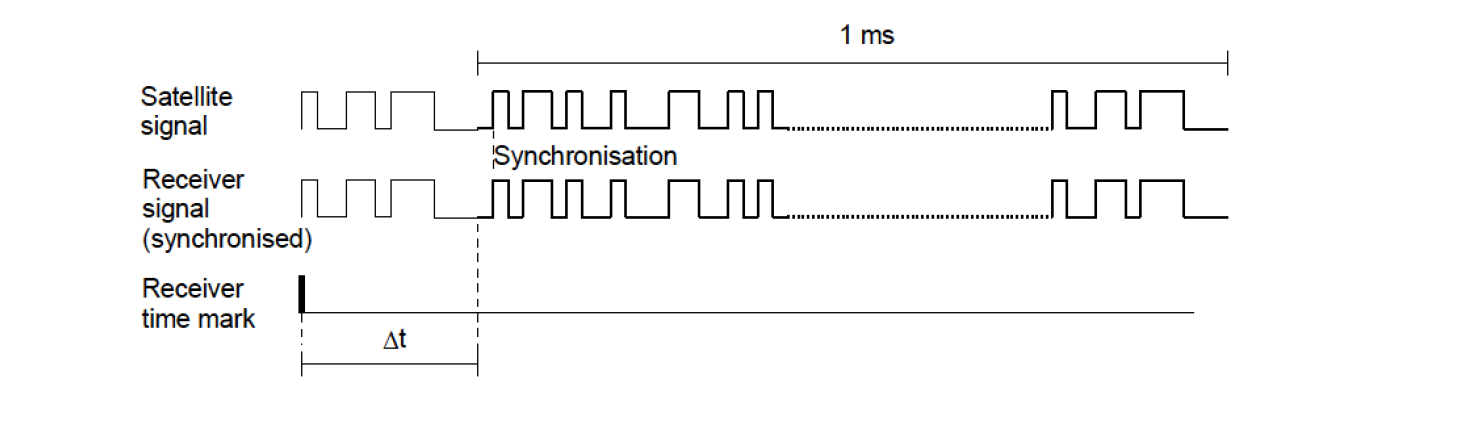
\includegraphics[width=\linewidth]{Figures/L4_arrival_time.PNG} 
\end{minipage}
\begin{minipage}{\linewidth}
    \centering      
    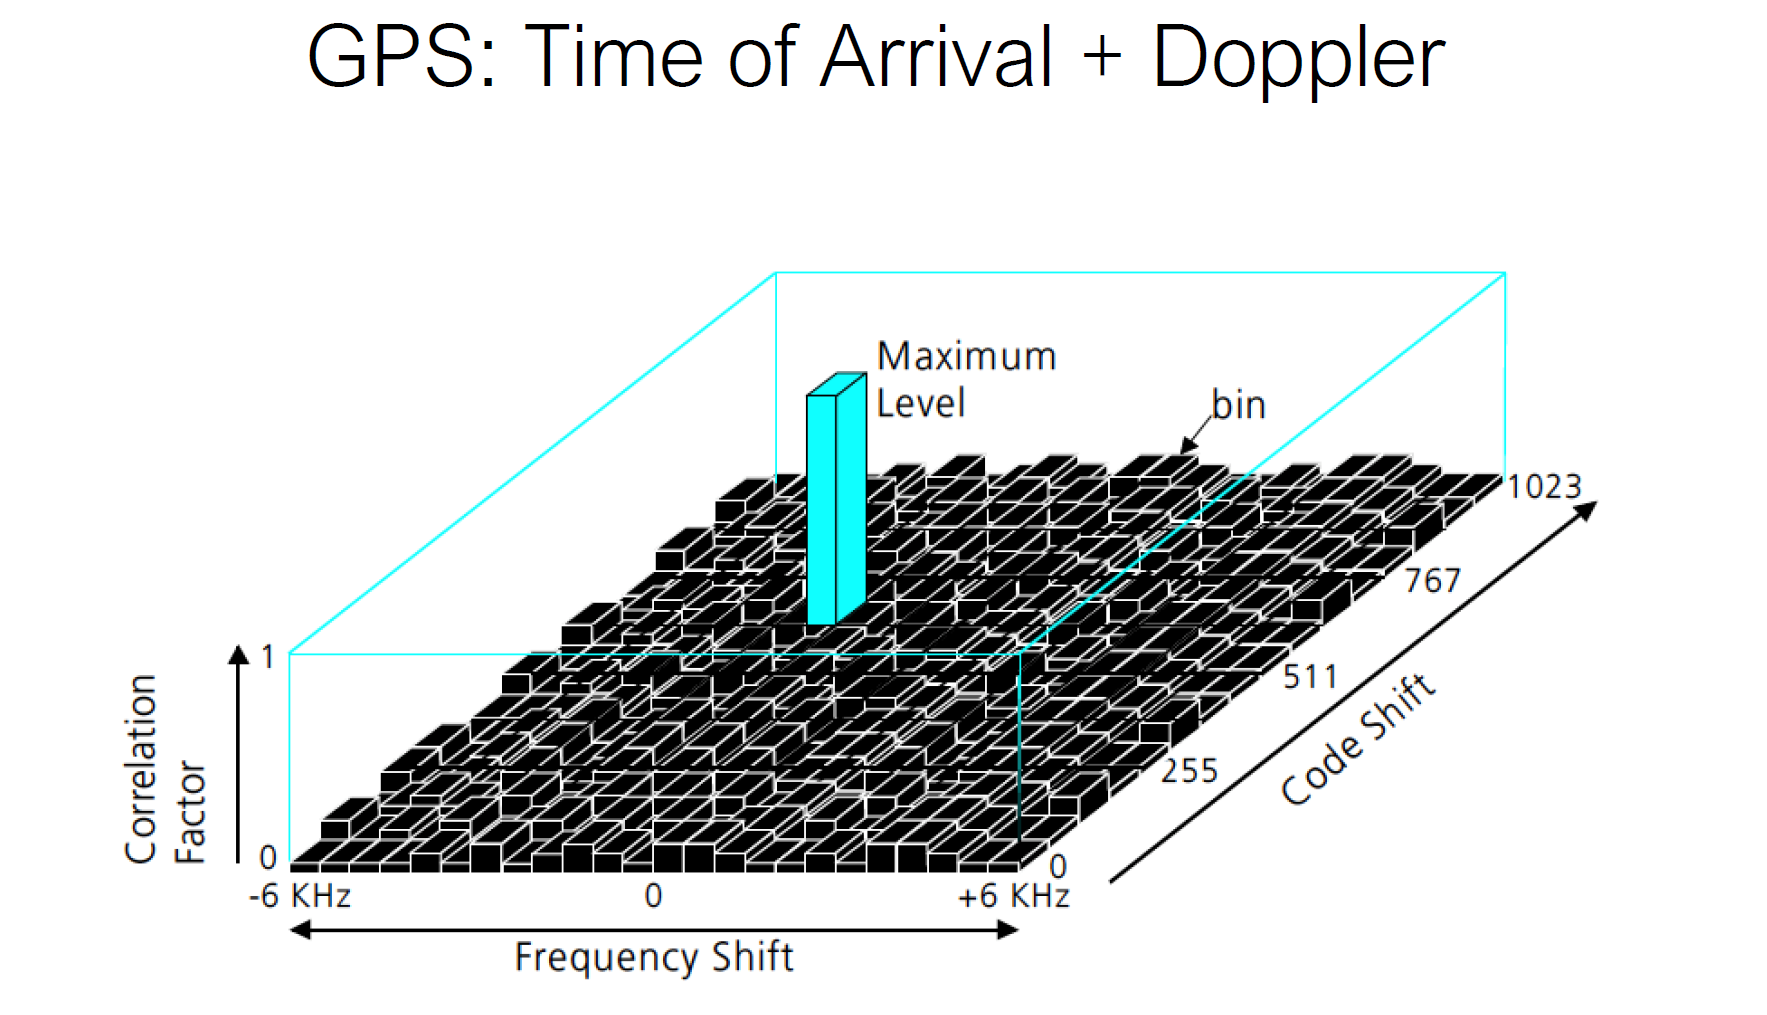
\includegraphics[width=\linewidth]{Figures/L4_signal_pane.PNG} 
\end{minipage}

We need to find best correlation between spreading code and received signal w.r.t. 2 dimensional signal. Along frequency shift (due to doppler effect that either squeezes or broadens signal, meaning increase or decrease frequency) and along code shift duet to synchronization of spreading code with received signal.

Received signal will be below thermal noise but despreaded signal will appear above noise level.

\begin{minipage}{\linewidth}
    \centering      
    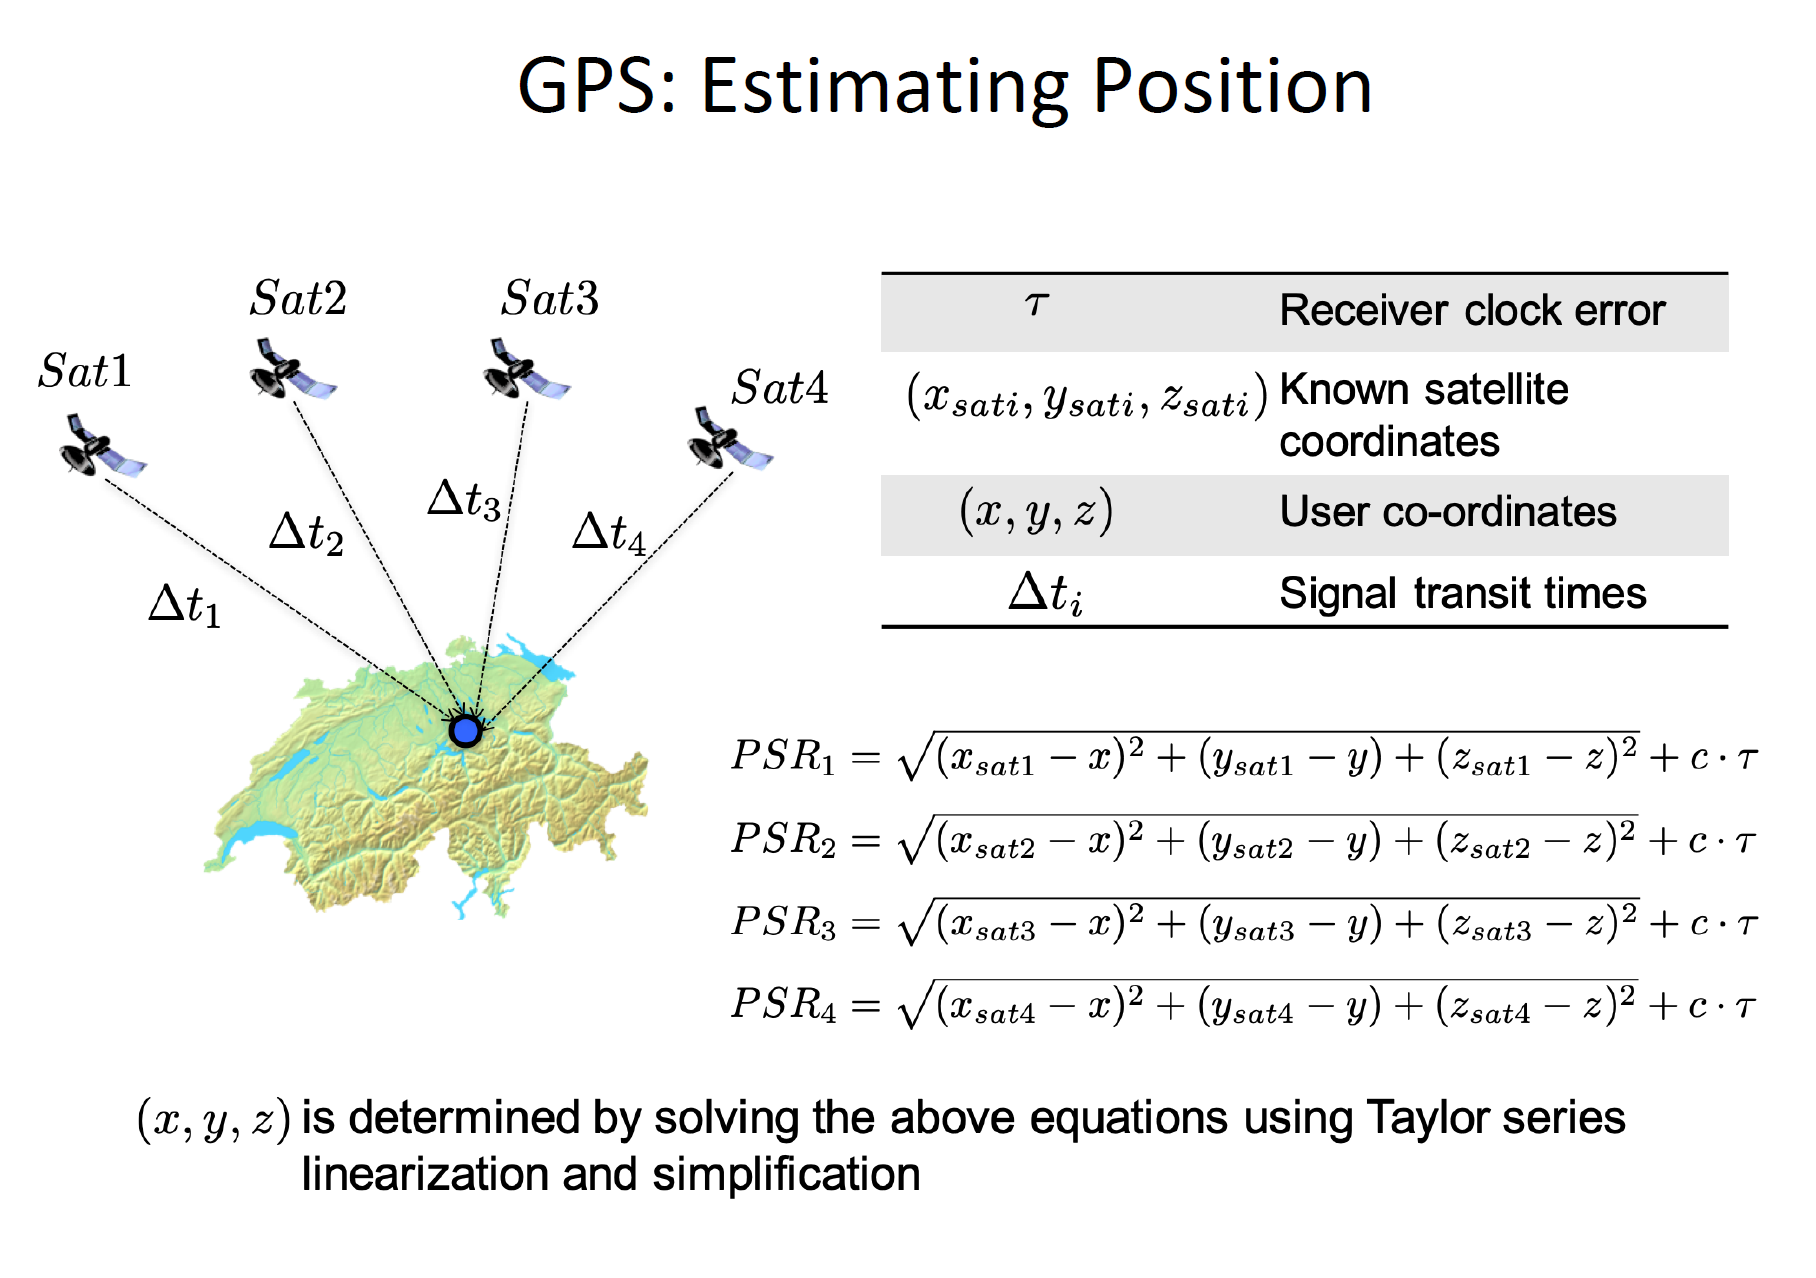
\includegraphics[width=\linewidth]{Figures/L4_positioning.PNG} 
\end{minipage}

\subsection{GPS Signal Spoofing Attack}
\begin{itemize}
    \item Attacker transmits specially crafted signals identical to sattellite signals but at higher power to overshadow legitimate satellite signals. But either modify navigation message contents or manipulate the time of arrival. 
    \item Receiver computes a false location base on the attackers spoofing signals
    \item There is an increasing availability of commercial GPS signal generators and low-cost radio hardware, which makes such an attack easy.
    \item Civilian GPS are not authenticated and can be generated OR delayed. Military GPS signals can only be delayed
\end{itemize}

\subsection{Detection and Mitigation of GPS Spoofing}
\paragraph{Countermeasures:} 
\begin{itemize}
    \item Infrastructure modifications: Adding cryptographic authentication to the navigation messages.
    \item Receiver end modifications:
    \begin{itemize}
        \item Spatial characteristics of the received signal (e.g. Angle of arrival, carrier phase measurements)
        \item Other physical-layer characteristics of the received GPS signals (received signal strength, AGC)
        \item Additional sensors or receivers to validate the estimated position, velocity and time.
    \end{itemize}
\end{itemize}

\paragraph{Angle of arrival:} is a function of the measured signal phase difference $\sigma$ at two close antennas and their separation D. 
\\
To mitigate spoofing attack, check if the signal truely comes from the direction where the satellite should be. Problem: Legitimate GPS signal may bounce of objects (multipathing) and thus not have expected angle and an attacker could use a drone to transmit the signal from there. And to reliably detect angle of arrival we need two antennas.

\paragraph{Monitoring Signal Characteristics:} Detect spoofing without changes to GPS, but monitoring of signal characteristics:
\begin{itemize}
    \item AGC, Noise level, nr. of satellites
    \item Autocorrelation Peak Distortion
    \item Spatial Diversity (AoA)
\end{itemize}

\subsubsection{SPREE - Spoofing Resistant GPS Receiver}
\begin{itemize}
    \item The first GPS receiver capable of detecting (up to an accuracy) all known spoofing attacks.
    \item A novel auxiliary peak tracking technique enables detection of a seamless takeover attacks (tracks all peaks).
    \item Perform some sanity checks on the peaks to detect if a peak is even possible or reasonable.
\end{itemize}

\begin{minipage}{\linewidth}
    \centering      
    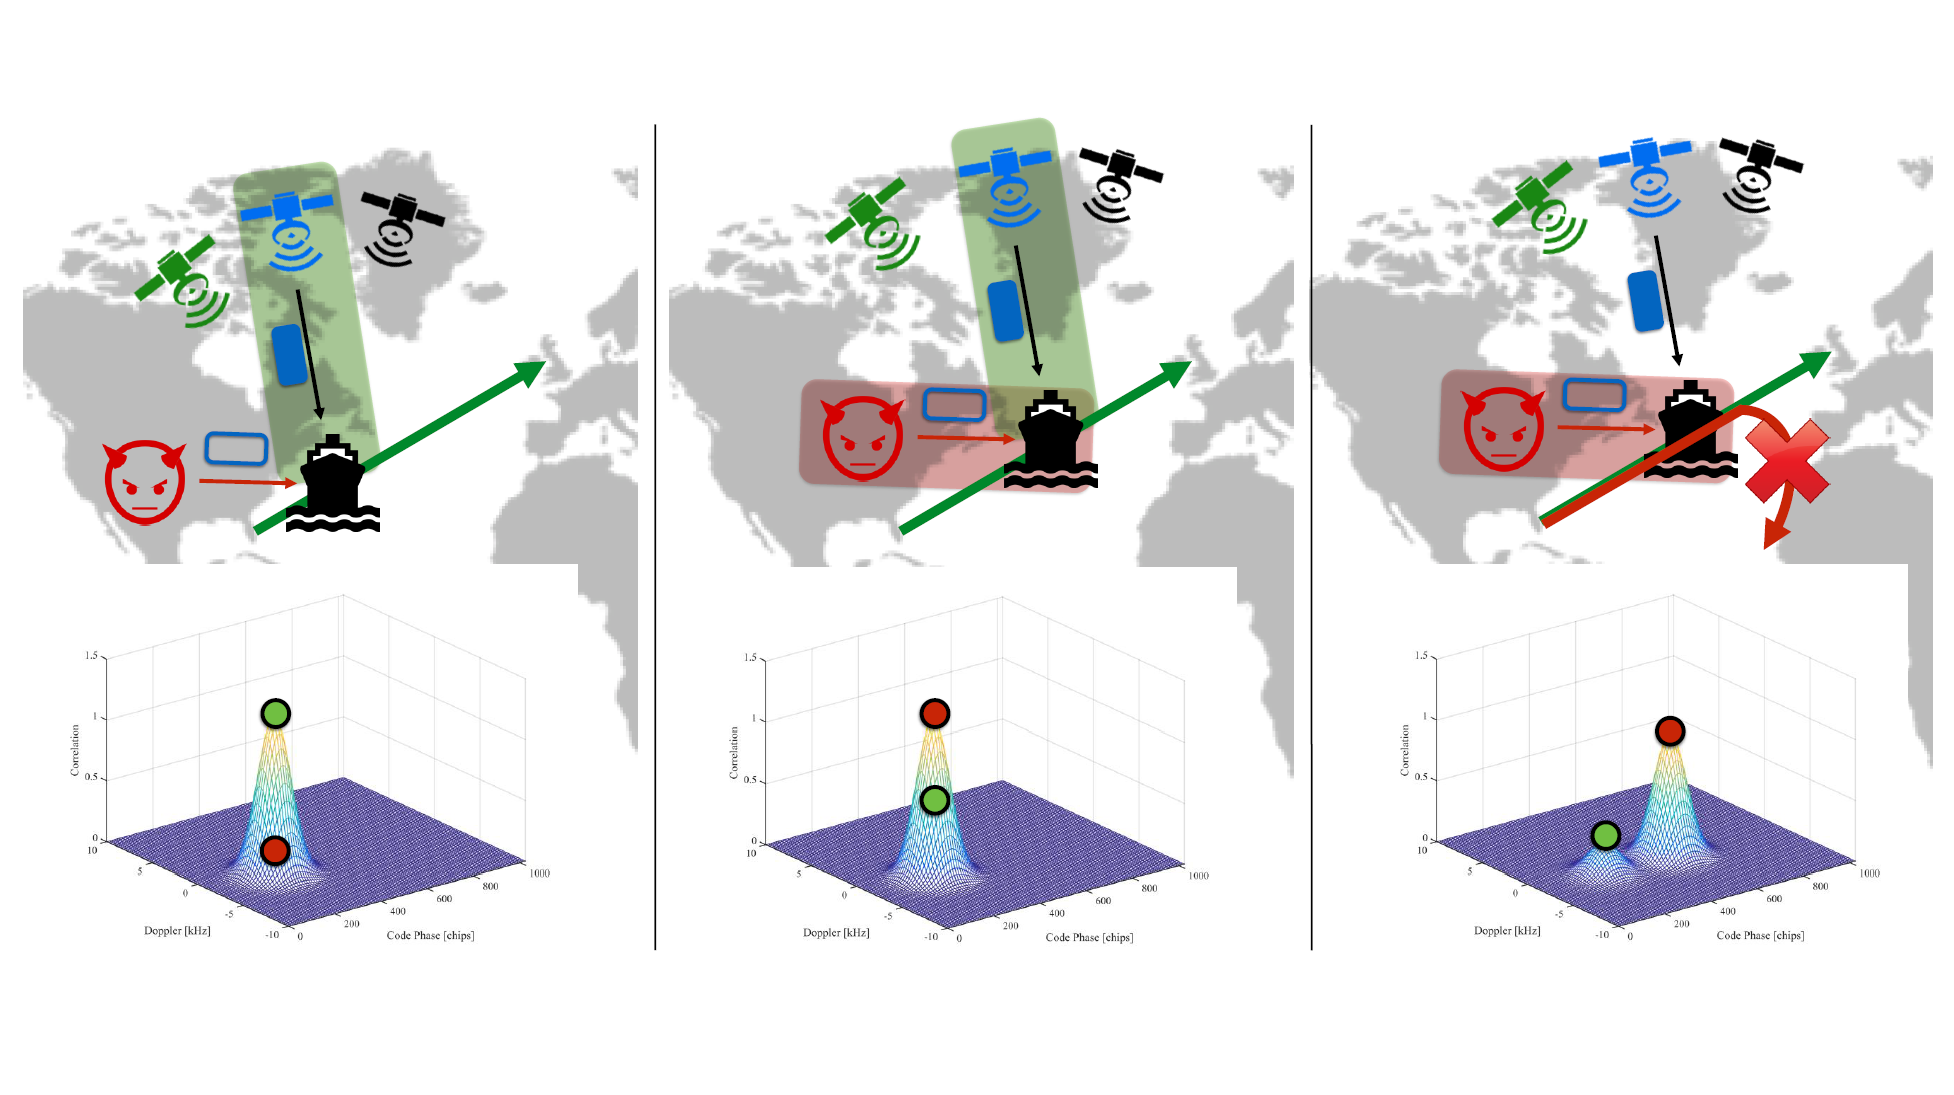
\includegraphics[width=0.9\linewidth]{Figures/L4_spree.PNG} 
\end{minipage}

\subsubsection{Leveraging Spatial Diversity}
\begin{minipage}{\linewidth}
    \centering      
    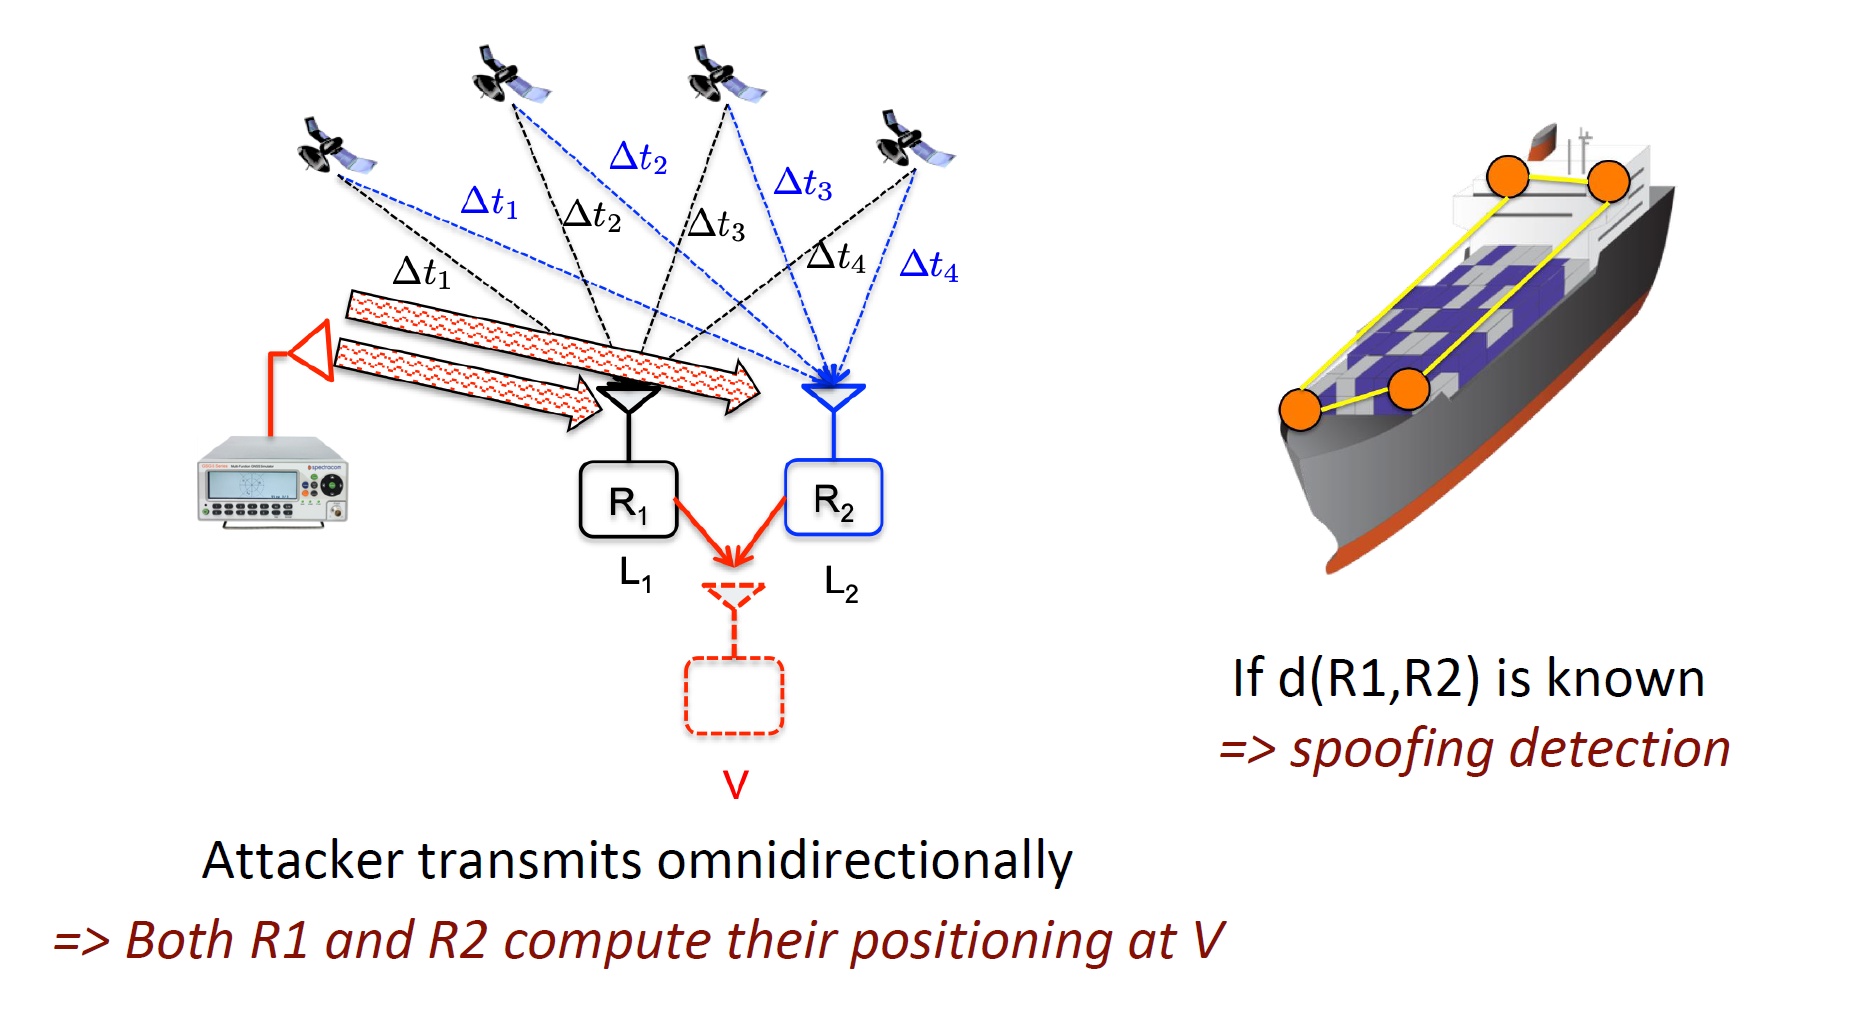
\includegraphics[width=0.9\linewidth]{Figures/L4_spatial.PNG} 
\end{minipage}

Test if positions of different antennas match up relatively to each other.
An attack now is still possible but it reduces the locations, where he can place spoofers (The GPS Group Spoofing Problem). The attacker needs to find GPS signals, transmission times and spoofer locations such that the location or time of each victim is spoofed to the desired location/time.
\\\\
Broadcast systems like GPS cannot be fully secured, this would require bidirectional communication or communication from the device to the infrastructure.

\subsubsection{Cryptographic Countermeasures}
\paragraph{Proposal for a Secure GPS (Kuhn):} Devices hold satellite public keys. At time t, a satellite uses a secret code to spread the navigation signal
\begin{itemize}
    \item The receiver uses a broadband receiver to receive the whole signal band (receiver does not know the despreading coe yet)
    \item At time t + dt, the satellite discloses its secret code, signed with its private key
    \item The receiver gets the code, verifies the signatures and despreads the signals.
    \item[-->] Prevents the generation of fake signals and their individual shifts.
    \item [-->] Prevents pulse-delay of individual signals, but not of aggregated signals (full band)
    \item there are some issues with its efficiency.
\end{itemize}